\documentclass[12pt]{article}
\usepackage[hidelinks]{hyperref}
\usepackage[a4paper]{geometry}
\usepackage[hang, labelfont=bf]{caption}
\usepackage{tikz}
\usepackage{float}
\usepackage{amsmath}
\usepackage{amssymb}
\usepackage{array}
\usepackage[ruled, vlined]{algorithm2e}

\DeclareMathOperator*{\bigforall}{\mbox{\Large $\mathsurround0pt \forall$}}
\newcommand*{\p}{\ensuremath{\mathcal{P}}}


\setlength{\parindent}{0pt}
\setlength{\parskip}{1ex}

\author{
    \textsc{Jakub Pawlak}\\
    \href{mailto:j.pawlak@student.fontys.nl}{\texttt{j.pawlak@student.fontys.nl}}
    \and 
    \textsc{Grzegorz Malisz}\\
    \href{mailto:g.malisz@student.fontys.nl}{\texttt{g.malisz@student.fontys.nl}}
}

\title{\sffamily\bfseries\Huge Peking express optimal-strategy algorithm}

\begin{document}

\begin{titlepage}
    \newgeometry{left=1in, right=1in}
    \maketitle
    \thispagestyle{empty}
    \tableofcontents
    \restoregeometry
\end{titlepage}
\setcounter{page}{2}

\section{Introduction}

In the game 2 players take turns traversing a directed weighted graph.
One vertex is chosen as a destination and the aim of the game is to be the first player to reach that vertex.

Each player starts with the same budget --- every vertex has an associated travel cost, and each time a player traverses that edge, their budget decreases by that amount.
Players can only traverse an edge if their current budget is higher than the cost associated with that edge.

Additionally, some of the graph's vertices are \emph{critical locations}, meaning that they can only accomodate one player at a time.

An example map is shown on the fig.~\ref*{fig:example-map} below.
The start location is node $A$, marked in green, the target is node $D$ shown in red,
and the critical locations are marked with a double border, in this case only one being node $C$.

\begin{figure}[H]\centering
    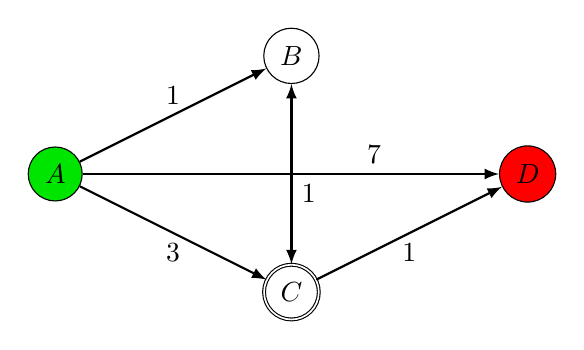
\begin{tikzpicture}[main/.style = {draw, circle}]
        \node[main, fill=green!90!black] (a) at (0,1.5) {$A$};
        \node[main, double] (c) at (3,0) {$C$};
        \node[main] (b) at (3,3) {$B$};
        \node[main, fill=red] (d) at (6,1.5) {$D$};

        \draw[-latex, thick] (a) -- (b) node[midway, above] {1};
        \draw[latex-latex, thick] (b) -- (c) node[midway, below right] {1};
        \draw[-latex, thick] (a) -- (c) node[midway, below] {3};
        \draw[-latex, thick] (a) -- (d) node[pos=0.7, above] {7};
        \draw[-latex, thick] (c) -- (d) node[midway, below] {1};
    \end{tikzpicture}
    \caption{Example map for the game with the source marked green and the target shown as red.}
    \label{fig:example-map}
\end{figure}

In each turn player can do one of the following:
\begin{enumerate}
    \item Travel to an adjacent vertex if the player's budget is higher than the cost of traversal
    \item Stay in the current location
\end{enumerate}

The assignment is to write an algorithm who will choose an optimal move given a game setting.

\section{Devising an algorithm}

\subsection{Resource constrained shortest path}

Consider a directed graph $G(V,E)$, where $V = \{v_1, \ldots , v_n\}$ represents a set of vertices,
and $E \subseteq \{ (i,j) \mid v_i \in V, v_j \in V, i \neq j \}$ a set of edges.
For each edge $(i,j) \in E$ there are 2 weights $c_{ij}$ and $t_{ij}$,
that represent the length and resource consumption of traversing the edge.

In the case of this game:
\begin{equation}
    \bigforall_{i,j} \; c_{ij} = 1
    \label{eq:all_cost_one}
\end{equation}
Because it takes just 1 turn to traverse an edge.

Consider a set $P$ of all simple paths possible in the graph $G$, and a set $P(S,T) \subset P$ of simple paths from $S$ (source) to $T$ (target).
For all $p \in P$ define the functions $C: P \to \mathbb{Z}^+$, and $R: P \to \mathbb{Z}^+$ as follows:
\begin{align}
    C(p) & = \sum\limits_{(i,j) \in p} c_{ij} \label{eq:len-func}  \\
    R(p) & = \sum\limits_{(i,j) \in p} t_{ij} \label{eq:cost-func}
\end{align}

The aim of the game is to reach the target in the shortest amount of moves while staying within the budget.
Therefore, we want to find such $p \in P(S,T)$ that minimizes the value of $C(p)$ while maintaing the condition $R(p) \leq t_{max}$.
This is the classic example of a well-known resource-constrained shortest path problem (RCSP).

\subsection{Critical location limitations}

\subsubsection{Blocking paths}

Now consider 2 simple paths: $p_a = (a_1, \ldots, a_n)$, and $p_b = (b_1, \ldots, b_k)$, where $a_n = b_k = T$, which is the target node.
They will denote the shortest path chosen by each player respectively.

Since the critical loactions can only host one player at the time,
if both of the paths contain some critical location $c$, the players can block each other.

Assume player $a$ moves first.

In this case, path $p_a$ will block $p_b$, which we will denote as $p_a \vdash p_b$, if the following condition is met:
\begin{equation}
    p_a \vdash p_b \iff \exists i : a_i = b_i = c
\end{equation}
The opposite can occur, that is path $p_b$ will block $p_a$, denoted $p_a \dashv p_b$ if
\begin{equation}
    p_a \dashv p_b \iff \exists i : a_i = b_{i-1} = c
\end{equation}
This equation is an obvious consequence of the one above it, because after making a move, the path of the first player will ``shift'' to the left,
resulting in situation where the second player will be in a blocking advantage.

Additionally, if both conditions occur,
the one that occured first has a precedence,
that is, for some critical $c_1, c_2$:
\begin{equation}
    \exists i,j : (a_i = b_i = c_1 \land a_j = b_{j-1} = c_2) \implies
    \begin{cases}
        p_a \vdash p_b, \quad \text{if $i < j$} \\
        p_a \dashv p_b, \quad \text{if $i > j$} \\
    \end{cases}
\end{equation}


\begin{figure}[H]\centering
    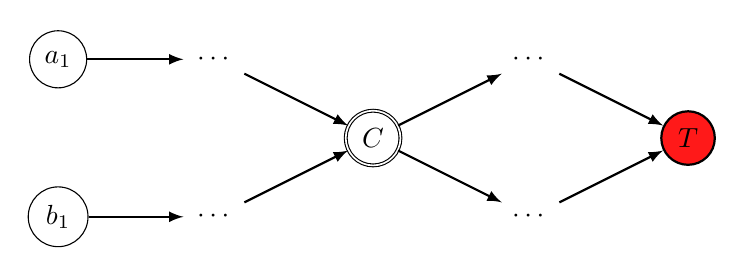
\begin{tikzpicture}[main/.style = {draw, circle}, ar/.style={thick, -latex}]
        % \node[main, fill=green!90!black] (start) at (0,0) {$S$};
        \node[main, double] (n) at (6,0) {$C$};
        \node[main, fill=red!90, thick] (target) at (10,0) {$T$};


        \node[main] (a1) at (2, 1) {$a_1$};
        \node[circle] (a2) at (4, 1) {$\cdots$};
        \node[circle] (a3) at (8, 1) {$\cdots$};

        \node[main] (b1) at (2, -1) {$b_1$};
        \node[circle] (b2) at (4, -1) {$\cdots$};
        \node[circle] (b3) at (8, -1) {$\cdots$};

        % \draw[ar] (start) -- (a1);
        \draw[ar] (a1) -- (a2);
        \draw[ar] (a2) -- (n);
        \draw[ar] (n) -- (a3);
        \draw[ar] (a3) -- (target);

        % \draw[ar] (start) -- (b1);
        \draw[ar] (b1) -- (b2);
        \draw[ar] (b2) -- (n);
        \draw[ar] (n) -- (b3);
        \draw[ar] (b3) -- (target);
    \end{tikzpicture}
    \caption{Illurtration of two paths that might block}
\end{figure}


\subsection{Solving RCSP problem}

This problem can be solved in 2 approaches:
starting from source to all of the nodes reachable from it,
or starting from the target, to all of the nodes it is reachable from.

Since thrroughout the game the starting positions would stay the same,
but the target node $n$ will be constant, we will use the second approach.

Let $z_n(a, t)$ be $\min \{ C(p) \mid p \in P(a,n), T(p) \leq t \}$.
Then, we can define it to be

\begin{align}
    z_n(n,t) & = 0                                             \\
    z_n(a,t) & = \infty \quad \text{if $a \neq n$ and $t < 0$} \\
    z_n(a,t) & =
    \min\limits_{i : \exists (a,i) \in E}
    \Big\{
    z_n(i, t - t_{ai})
    \Big\}
\end{align}

This can be easily calculated using the dynamic programming approach, by filling in the table like the following:

\begin{table}\centering
    \begin{tabular}{|c|c c c c c c|}
        \hline
            & 0        & 1        & 2        & 3 & 4 & 5 \\ \hline
        $A$ & $\infty$ & $\infty$ & $\infty$ & 3 & 2 & 2 \\
        $B$ & $\infty$ & $\infty$ & 2        & 2 & 2 & 2 \\
        $C$ & $\infty$ & 1        & 1        & 1 & 1 & 1 \\
        $D$ & 0        & 0        & 0        & 0 & 0 & 0 \\ \hline
    \end{tabular}
    \caption{Example $z$ table for example from fig.~\ref{fig:example-map}}
\end{table}

Since each of the values of $z_n$ depends only on values for smaller $t$, we can fill this table going column-by-column.
The following algorithm accomplishes exactly that:

\begin{algorithm}[H]
    \DontPrintSemicolon
    \KwData{Directed graph $G(V,E)$,
        a set of weights $t_{ij}$ for each edge $i \to j$,
        target location $n$,
        and starting budget $t_{max}$}
    \KwResult{A table $Z$ such that $Z[a][t] = z_n(a,t)$}
    \BlankLine
    \Begin {
        \For{$t = 0$ \KwTo $t_{max}$}{
            $Z[n][t] \longleftarrow 0$\;
            \ForEach{$a \in V, a \neq n$}{
                $N \longleftarrow \emptyset$\;
                \ForEach{$b \in V$, such that $(a,b) \in E$}{
                    \If{$t_{ab} \leq t$}{
                        $l \longleftarrow Z[b][t - t_{ab}] + 1$\;
                        add $l$ to $N$\;
                    }
                }
                \eIf{$N = \emptyset$}{
                    $Z[a][t] \longleftarrow \infty$\;
                }{
                    $Z[a][t] \longleftarrow \min(N)$\;
                }
            }
        }
    }
    \caption{Algorithm to fill the table of $z_n(a,t)$}
\end{algorithm}

\subsection{Optimal strategy}

\subsubsection{Generating the shortest paths}

Let $\p(a,t)$ denote a set of all shortest paths constrained by maximum resource usage $t$.
That is
\begin{equation*}
    \p(a,t) = \big\{ p \in P(a,t) \mid C(p) = z(a,t) \big\}
\end{equation*}
Since all of these paths are the shortest, all of them have the same length equal to $z(a,t)$.

\begin{equation}
    N(a,t) = \big\{ n \mid (a,n) \in E , z(n,t-t_{an}) < z(a, t) \big\}
\end{equation}

\begin{equation}
    \p(a,t) =
    \begin{cases}
        \big\{ (T) \big\}, \quad \text{if $a = T$}     \\[1ex]
        \;\emptyset, \quad \text{if $z(a,t) = \infty$} \\[1ex]
        \bigcup\limits_{n \in N(a,t)} \Big\{ a::p \mid p \in \p(n,t-t_{an}) \Big\}
    \end{cases}
\end{equation}

Where $a :: p$ will denote path of taking $a$, followed by path $p$.
Formally:
\begin{equation*}
    a :: (p_1, p_2, \ldots, p_n) = (a, p_1, p_2, \ldots, p_n)
\end{equation*}

\begin{algorithm}[H]
    \DontPrintSemicolon
    \SetKwFunction{FPaths}{Paths}
    \SetKwFunction{FCombine}{Combine}
    \SetKwProg{Fn}{Function}{:}{}
    \KwData{Directed graph $G(V,E)$,
        a set of weights $t_{ij}$ for each edge $i \to j$,
        target location $n$,
        starting position $a$
        and starting budget $t$}
    \KwResult{A set $\p(a,t)$ of shortest paths from $a$ to $n$ not exceeding the budget $t$}
    \BlankLine
    \Fn{\FPaths{$a,t$}}{
    \uIf{$a = n$}{
        \KwRet{$\{(n)\}$}\;
    }
    \uElseIf{$t \leq 0$}{
        \KwRet{$\emptyset$}\;
    }
    \Else{
    \ForEach{$b \in V$, such that $(a,b) \in E$}{
    $R \longleftarrow = \emptyset$\;
    \If{$z_n(b, t-t_{ab}) < z_n(a,t)$}{
    $P \longleftarrow \FPaths{a,t}$\;
    \ForEach{$p \in P$}{
        $p' \longleftarrow \FCombine{a,p}$\;
        add $p'$ to $R$
    }
    }
    }
    \KwRet{$R$}\;
    }
    }
    \caption{Algorithm for generating all of the available shortest paths within a budget}
\end{algorithm}

\subsubsection{Choosing the best path}

\end{document}